\documentclass[tikz,border=10pt]{standalone}
\newcommand{\comment}[1]{}

\usepackage{tikz}
\usepackage[utf8]{inputenc}
\usepackage{verbatim}
\usepackage{amsmath}

\usetikzlibrary{shadows,patterns,snakes}
\usetikzlibrary{intersections}
\usetikzlibrary{positioning}
\usetikzlibrary{calc}

\begin{document}
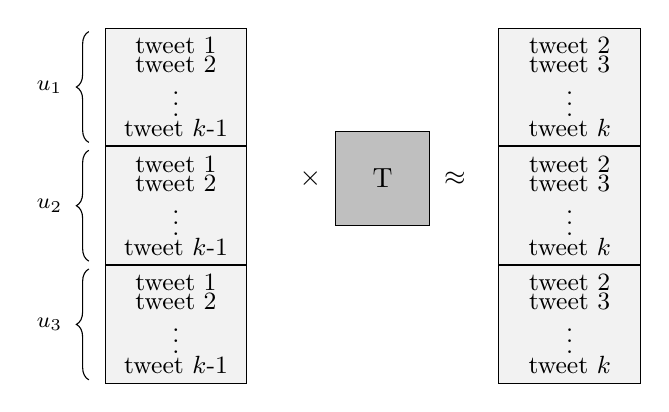
\begin{tikzpicture}

\tikzstyle{userBox}=[rectangle,anchor=north west,align=center,minimum width=1.8cm,minimum height=0.8cm,draw=black,fill=black!5!white,font=\fontsize{0.3cm}{0.1cm}\selectfont];
\tikzstyle{tBox}=[rectangle,anchor=north west,align=center,minimum size=1.2cm,draw=black,fill=black!25!white];
%\tikzstyle{userBox}=[rectangle, minimum size=1.0cm,draw=red,fill=red!25,rounded corners,align=center,inner sep=0.2cm, font=\fontsize{0.5cm}{0.2cm}\selectfont];

\coordinate (curr) at (0,0);

%\node [userBox] (curr) at (curr.south west) {tweet 1\\tweet 2\\$\vdots$\\tweet $n$};

\foreach \u in {1,...,3}{
	\node [userBox] (curr) at (curr.south west) {tweet 1\\tweet 2\\$\vdots$\\tweet $k$-1};
	
	\draw [decorate,decoration={brace,amplitude=4.5pt},xshift=-0cm,yshift=-0pt] ($(curr.south west)+(-0.2,0.05)$) -- ($(curr.north west)+(-0.2,-0.05)$) node [black,midway,xshift=-0.5cm] {\footnotesize $u_\u$};	

};
		

\coordinate (curr) at (5,0);

%\node [userBox] (curr) at (curr.south west) {tweet 1\\tweet 2\\$\vdots$\\tweet $n$};

\foreach \u in {1,...,3}{
	\node [userBox] (curr) at (curr.south west) {tweet 2\\tweet 3\\$\vdots$\\tweet $k$};
	
	%\draw [decorate,decoration={brace,amplitude=4.5pt},xshift=-0cm,yshift=-0pt] (curr.south west) -- (curr.north west) node [black,midway,xshift=-0.5cm] {\footnotesize $u_\u$};	

};

\node (times) at ($(curr.north east)+(-4.2,1.1)$) {$\times$};
\node [tBox, right =0.05cm of times] (matrix) {T};
\node [right=0.05cm of matrix] (approx) {$\approx$};

\end{tikzpicture}
\end{document}
